%!TEX root = ../../template.tex
%%%%%%%%%%%%%%%%%%%%%%%%%%%%%%%%%%%%%%%%%%%%%%%%%%%%%%%%%%%%%%%%%%%%
%% data_model_implementation.tex
%% Data Model and Storage Details section for Implementation chapter
%%%%%%%%%%%%%%%%%%%%%%%%%%%%%%%%%%%%%%%%%%%%%%%%%%%%%%%%%%%%%%%%%%%%

\section{Data Model and Storage Details}
\label{sec:DataModelImplementation}

This section describes the schema definitions for the platform's data model. The reasoning behind choosing TimescaleDB, the dual-schema layout, and the typed-based value columns approach are covered in Section~\ref{sec:ProposedModelDataModelAndStorageDesign}.

\subsection{Metadata Schema}
The \texttt{reg} schema holds the relational tables for the platform's core entities: users, devices, data keys, monitoring rules, anomaly detector configurations, notification preferences, and sent notifications. These tables use standard relational patterns with foreign key constraints that enforce the ownership hierarchy. Figure~\ref{fig:database-reg-schema} shows the full entity relationship diagram for this schema.

\begin{figure}[htbp]
    \centering
    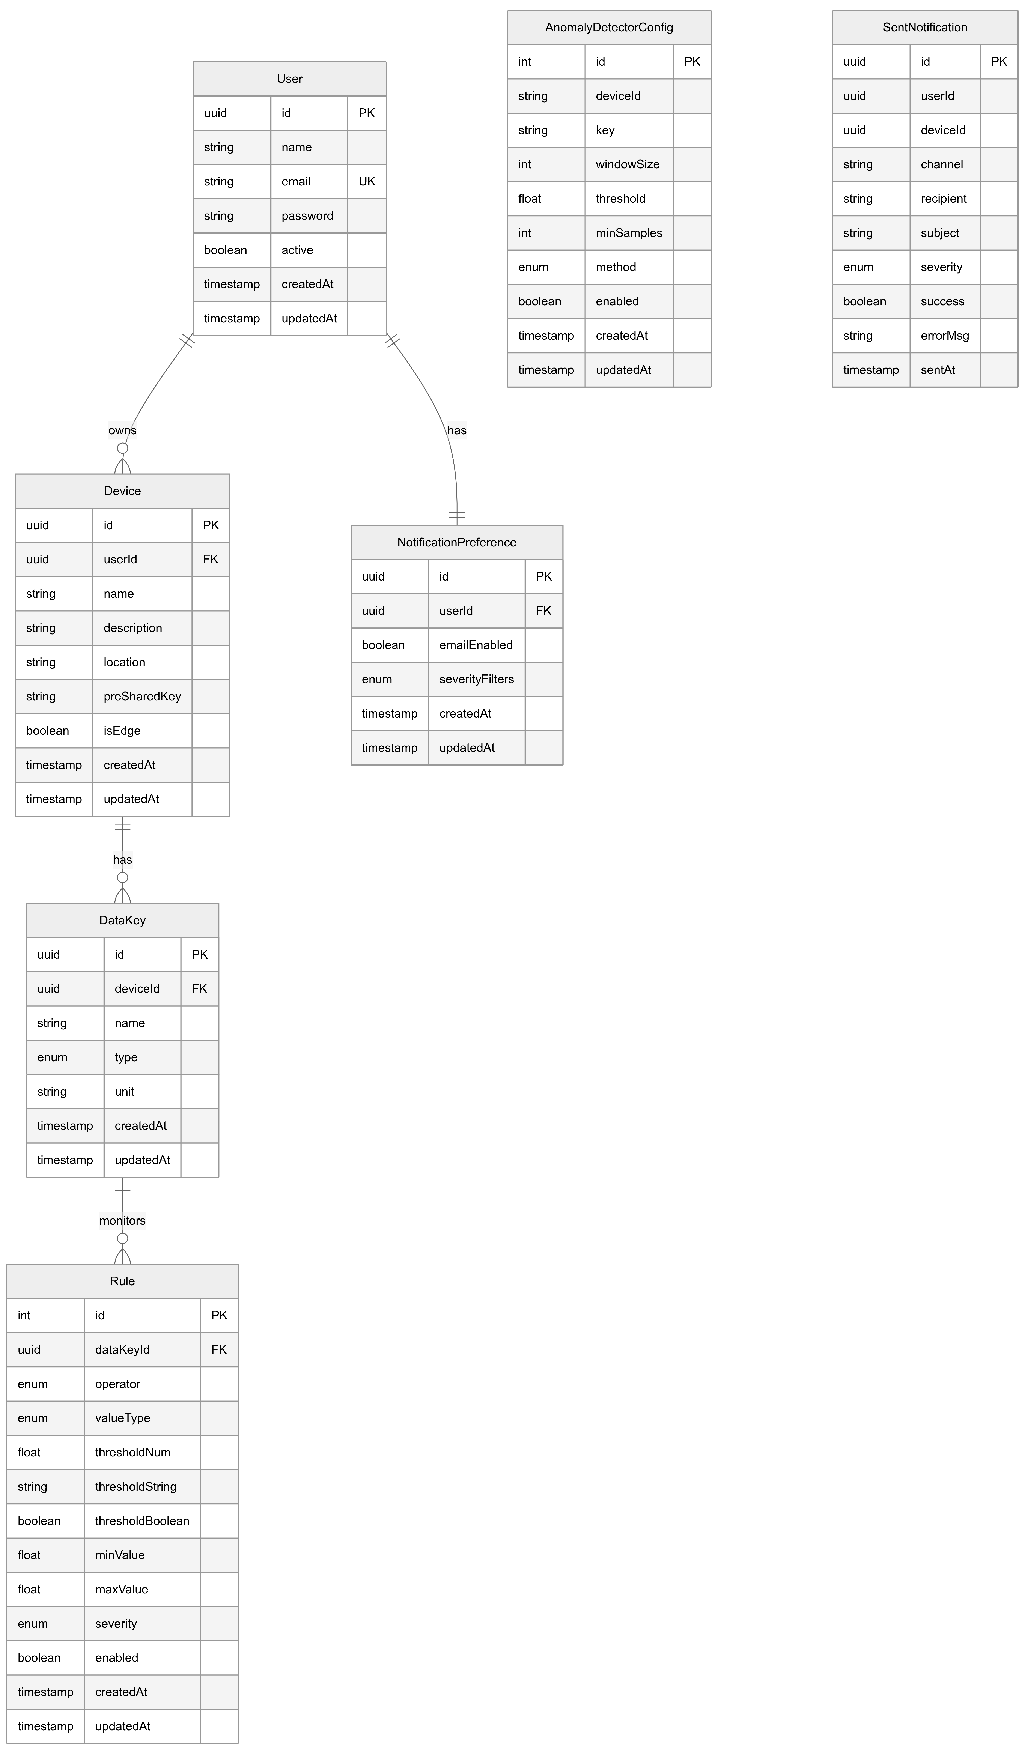
\includegraphics[height=\textheight, keepaspectratio]{Chapters/Figures/Databases/Implemented/regSchema.pdf}
    \caption{Entity relationship diagram for the \texttt{reg} (metadata) schema.}
    \label{fig:database-reg-schema}
\end{figure}

\subsubsection{Users}
The User table stores the platform's user accounts. Each user is identified by a \gls{UUID} primary key and has a name, email, and hashed password. The active flag allows disabling accounts without deleting them. This table is the root of the ownership hierarchy. Devices belong to users, and through devices, all downstream entities (data keys, rules, alerts) are indirectly owned by a user.

\subsubsection{Devices}
The Device table represents registered \gls{IoT} devices. Each device belongs to exactly one user through the \texttt{user\_id} foreign key and has descriptive metadata: a name, an optional description, and an optional location.

The \texttt{pre\_shared\_key} column stores the credential used during the first step of the device authentication flow, as described in Section~\ref{sec:ServiceImplementationDetails}. The \texttt{is\_edge} boolean field marks whether the device connects through an edge node rather than directly to the cloud \gls{MQTT} broker. Devices with \texttt{is\_edge = true} receive \gls{JWT} tokens containing an \texttt{isEdge} claim, which the edge node's local Mosquitto broker uses for authentication. Timestamps track when the device was registered and last updated.

\subsubsection{Data Keys}
The DataKey table records the telemetry fields that each device has already sent to the platform. Each entry has a \gls{UUID} primary key and is linked to a device through the \texttt{deviceId} foreign key. The \texttt{name} column holds the field name as extracted during ingestion, \texttt{type} records its data type (number, boolean, or string), and the optional \texttt{unit} column allows annotating the field with a measurement unit. A unique constraint on the combination of device and name ensures each telemetry field is registered only once per device.

Data keys are created automatically by the Metadata Service as it consumes the normalized telemetry stream. They serve as the binding point for monitoring rules: a rule can only be defined against a known data key.

\subsubsection{Rules}
The Rule table stores monitoring rules defined by the user. Each rule is linked to a data key through \texttt{dataKeyId}. The \texttt{operator} column defines the comparison to perform on the incoming data.

Thresholds follow a polymorphic pattern: three nullable columns (\texttt{threshold\_num}, \texttt{threshold\_string}, \texttt{threshold\_boolean}) handle different value types, with only the column matching the rule's \texttt{valueType} filled in. For range operators, \texttt{min\_value} and \texttt{max\_value} define the limits. The \texttt{enabled} flag lets users temporarily disable a rule without deleting it.

The \texttt{severity} column uses the \texttt{RuleSeverity} enum with four levels: \texttt{CRITICAL}, \texttt{HIGH}, \texttt{MEDIUM}, and \texttt{LOW}. This field serves two purposes. It communicates the urgency of resulting alerts to users, and it determines if the rule is evaluated at the edge node, since only \texttt{CRITICAL} rules are synchronized to edge nodes for local evaluation (Section~\ref{sec:EdgeNode}).

\subsubsection{Anomaly Detector Configuration}
The \texttt{AnomalyDetectorConfig} table in the \texttt{reg} schema stores the settings for the statistical anomaly detection engine. Each record targets a specific scope, defined by a \texttt{deviceId} and a \texttt{key} column, both of which default to \texttt{"*"} as a wildcard. The detection parameters are \texttt{windowSize} (default 100), \texttt{threshold} (default 3.0), \texttt{minSamples} (default 30), and a \texttt{method} enum (currently only \texttt{Z\_SCORE}). An \texttt{enabled} boolean lets users turn detection on or off per scope. A unique constraint on \texttt{[deviceId, key]} ensures only one configuration exists for each scope.

The wildcards create a hierarchical lookup. When evaluating a data point, the Analytics Service picks the most specific match: it checks for an exact device-key pair first, then a device-wide wildcard, then a key-wide wildcard, and finally a global default where both fields are \texttt{"*"}. This lets users set platform-wide defaults and override them for specific devices or telemetry keys that behave differently.

\subsubsection{Notification Preference}
The \texttt{NotificationPreference} table controls how each user receives alert notifications. It has a \gls{UUID} primary key, a unique \texttt{userId} foreign key, an \texttt{emailEnabled} boolean (default true), and a \texttt{severityFilters} array of \texttt{RuleSeverity} values that defaults to all four levels. The unique constraint on \texttt{userId} means each user can only have one preference record. Cascade deletion removes it automatically when the user is deleted.

\subsubsection{Sent Notification}
The \texttt{SentNotification} table logs every notification delivery attempt. Each record stores the \texttt{userId}, \texttt{deviceId}, a \texttt{channel} string (defaulting to \texttt{"email"}), the \texttt{recipient} address, the email \texttt{subject}, and the alert \texttt{severity}. A \texttt{success} boolean and a nullable \texttt{errorMsg} column track whether the delivery worked and, if not, what went wrong. A \texttt{sentAt} timestamp records when the attempt happened. This gives operators a way to check delivery history and diagnose failures without digging through application logs.

\subsection{Time-Series Schema}
The \texttt{telemetry} schema contains the DeviceData hypertable and the Alert table. Figure~\ref{fig:database-telemetry-schema} shows the entity relationship diagram for this schema, including the foreign key references to the \texttt{reg} schema entities.

\begin{figure}[htbp]
    \centering
    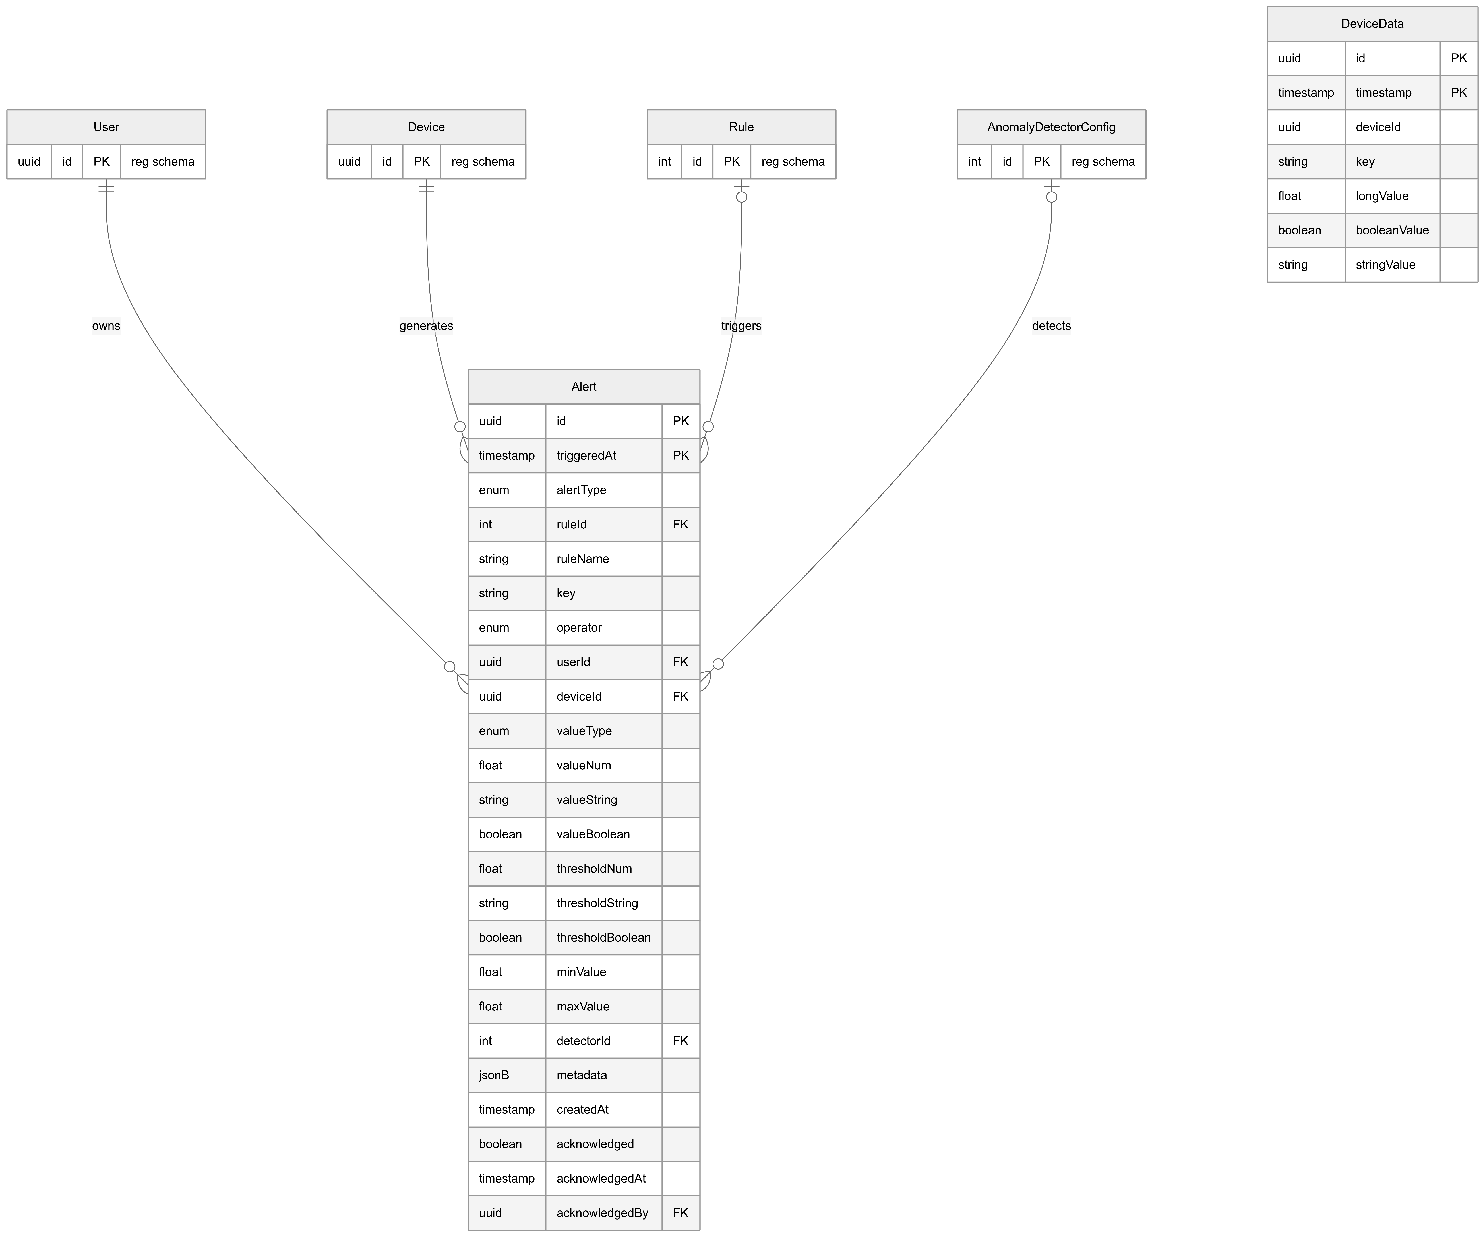
\includegraphics[width=\textwidth, keepaspectratio]{Chapters/Figures/Databases/Implemented/telemetrySchema.pdf}
    \caption{Entity relationship diagram for the \texttt{telemetry} schema, with references to the \texttt{reg} schema.}
    \label{fig:database-telemetry-schema}
\end{figure}

The DeviceData table is the main telemetry store. Each row holds a single data point: a value from a specific device at a specific time, identified by a device identifier, a timestamp, and a key name. The Storage Service writes these rows after consuming normalized telemetry from \texttt{telemetry.events}. The table is set up as a TimescaleDB hypertable partitioned on the \texttt{timestamp} column, so the database automatically splits data into time-based chunks for faster storage and querying.

Values are stored using three nullable columns: \texttt{long\_value} for numbers, \texttt{boolean\_value} for booleans, and \texttt{string\_value} for strings. Only the column matching the data point's type is filled in. The rest stay null.

The Alert table stores both rule-based threshold violations and statistical anomalies. Each alert saves a snapshot of the conditions when it was triggered: the rule name, data key, operator, threshold values, and the value that triggered it. The triggering value follows the same polymorphic pattern as the Rule table, with three nullable columns (\texttt{valueNum}, \texttt{valueString}, \texttt{valueBoolean}) and a \texttt{valueType} discriminator. Because the alert keeps its own copy of these fields, the record stays complete even if the original rule or detector is later changed or deleted.

These records are persisted by the Storage Service after it consumes \texttt{alerts.events}. This keeps alert storage aligned with the same event stream used for WebSocket delivery and notifications.

The primary key is a composite of \texttt{(id, triggeredAt)}, which allows TimescaleDB to partition the table on the trigger timestamp. Foreign keys to Rule, AnomalyDetectorConfig, and the acknowledging user use set-null deletion, so the alert survives if any of those records are removed. Foreign keys to the owning user and device use cascade deletion instead, since an alert without its owner or device has no meaning.

The table also tracks acknowledgment. An \texttt{acknowledged} flag, an \texttt{acknowledgedAt} timestamp, and an \texttt{acknowledgedBy} user reference let the web application show which alerts have been viewed.

An \texttt{alertType} enum separates the two detection methods: \texttt{RULE\_BASED} for threshold alerts (the default) and \texttt{STATISTICAL\_ANOMALY} for Z-score detections. Anomaly alerts include a \texttt{detectorId} foreign key to the \texttt{AnomalyDetectorConfig} table and a \texttt{metadata} \gls{JSON} column that stores the statistical context at detection time: mean, standard deviation, Z-score, window size, and threshold. Rule-based alerts leave these fields null. This way, both types of alerts share the same table, delivery pipeline, and acknowledgment flow while still carrying the context needed to understand how each one was generated.

\subsection{Indexing and Optimization}
The indexing strategy follows the main query patterns of the platform. The goal is simple: keep the most common reads fast without adding unnecessary indexes to write-heavy tables.

For the \texttt{DeviceData} hypertable, the main access pattern is retrieving the history of one telemetry key for one device. For that reason, the table has a composite index on \texttt{(device\_id, key)}. A second index on \texttt{timestamp DESC} helps with time-based queries, especially when the application requests the most recent values first. TimescaleDB also improves these queries through chunk exclusion, since chunks outside the requested time range do not need to be scanned.

The \texttt{Alert} table is indexed according to the filters exposed by the Read Service \gls{REST} \gls{API}. The index on \texttt{(userId, createdAt DESC)} supports the default alert list for each user, ordered by the most recent. The index on \texttt{(deviceId, createdAt DESC)} supports filtering alerts by device. Another index on \texttt{(userId, acknowledged)} helps separate pending alerts from acknowledged ones in the dashboard. Finally, the index on \texttt{ruleId} supports queries that fetch all alerts generated by a given rule.

\subsection{Edge Local Storage Schema}
The edge node uses SQLite with three tables, managed through a separate Prisma schema (Figure~\ref{fig:edge-sqlite-schema}).

The \texttt{device\_data} table buffers telemetry before it is sent to the cloud. Each row stores an identifier, the device identifier, the key name, a \texttt{value\_type} field, three nullable value columns (\texttt{num\_value}, \texttt{bool\_value}, \texttt{str\_value}), a floating-point timestamp, and a \texttt{synced} flag. This table is used as a local queue when the edge node cannot forward data immediately.

The \texttt{alerts} table stores alerts generated at the edge. Each row references a rule, identifies the device, user, and telemetry key, and stores the operator, a serialized \texttt{threshold} value, polymorphic value columns that follow the same pattern as \texttt{device\_data}, a \texttt{triggered\_at} timestamp, a \texttt{payload} JSON string, and a \texttt{synced} flag. This allows the edge node to keep alerts locally until they are delivered to the cloud.

The \texttt{rules} table stores the cached copy of the \texttt{CRITICAL} rules synchronized from the cloud. Each entry keeps the cloud rule identifier, the device, the data key, the operator, the value type, the threshold columns (\texttt{threshold\_num}, \texttt{threshold\_str}, \texttt{threshold\_bool}), optional range limits (\texttt{min\_value}, \texttt{max\_value}), the owning user, and an \texttt{updated\_at} timestamp.

% Figure: edge-sqlite-schema.png
% Should show three tables:
% 1. device_data: id (TEXT PK), device_id (TEXT), timestamp (REAL), key (TEXT),
%    value_type (TEXT), num_value (REAL nullable), bool_value (INT nullable),
%    str_value (TEXT nullable), synced (INT default 0). Index on (synced, timestamp).
% 2. alerts: id (TEXT PK), rule_id (INT), device_id (TEXT), user_id (TEXT default ""),
%    key (TEXT), value_type (TEXT), num_value (REAL nullable), bool_value (INT nullable),
%    str_value (TEXT nullable), operator (TEXT), threshold (TEXT nullable),
%    triggered_at (REAL), payload (TEXT default "{}"), synced (INT default 0).
%    Index on (synced, triggered_at).
% 3. rules: id (INT PK), device_id (TEXT), data_key (TEXT), operator (TEXT),
%    value_type (TEXT), threshold_num (REAL nullable), threshold_str (TEXT nullable),
%    threshold_bool (INT nullable), min_value (REAL nullable), max_value (REAL nullable),
%    user_id (TEXT default ""), updated_at (REAL).
\begin{figure}[htbp]
    \centering
    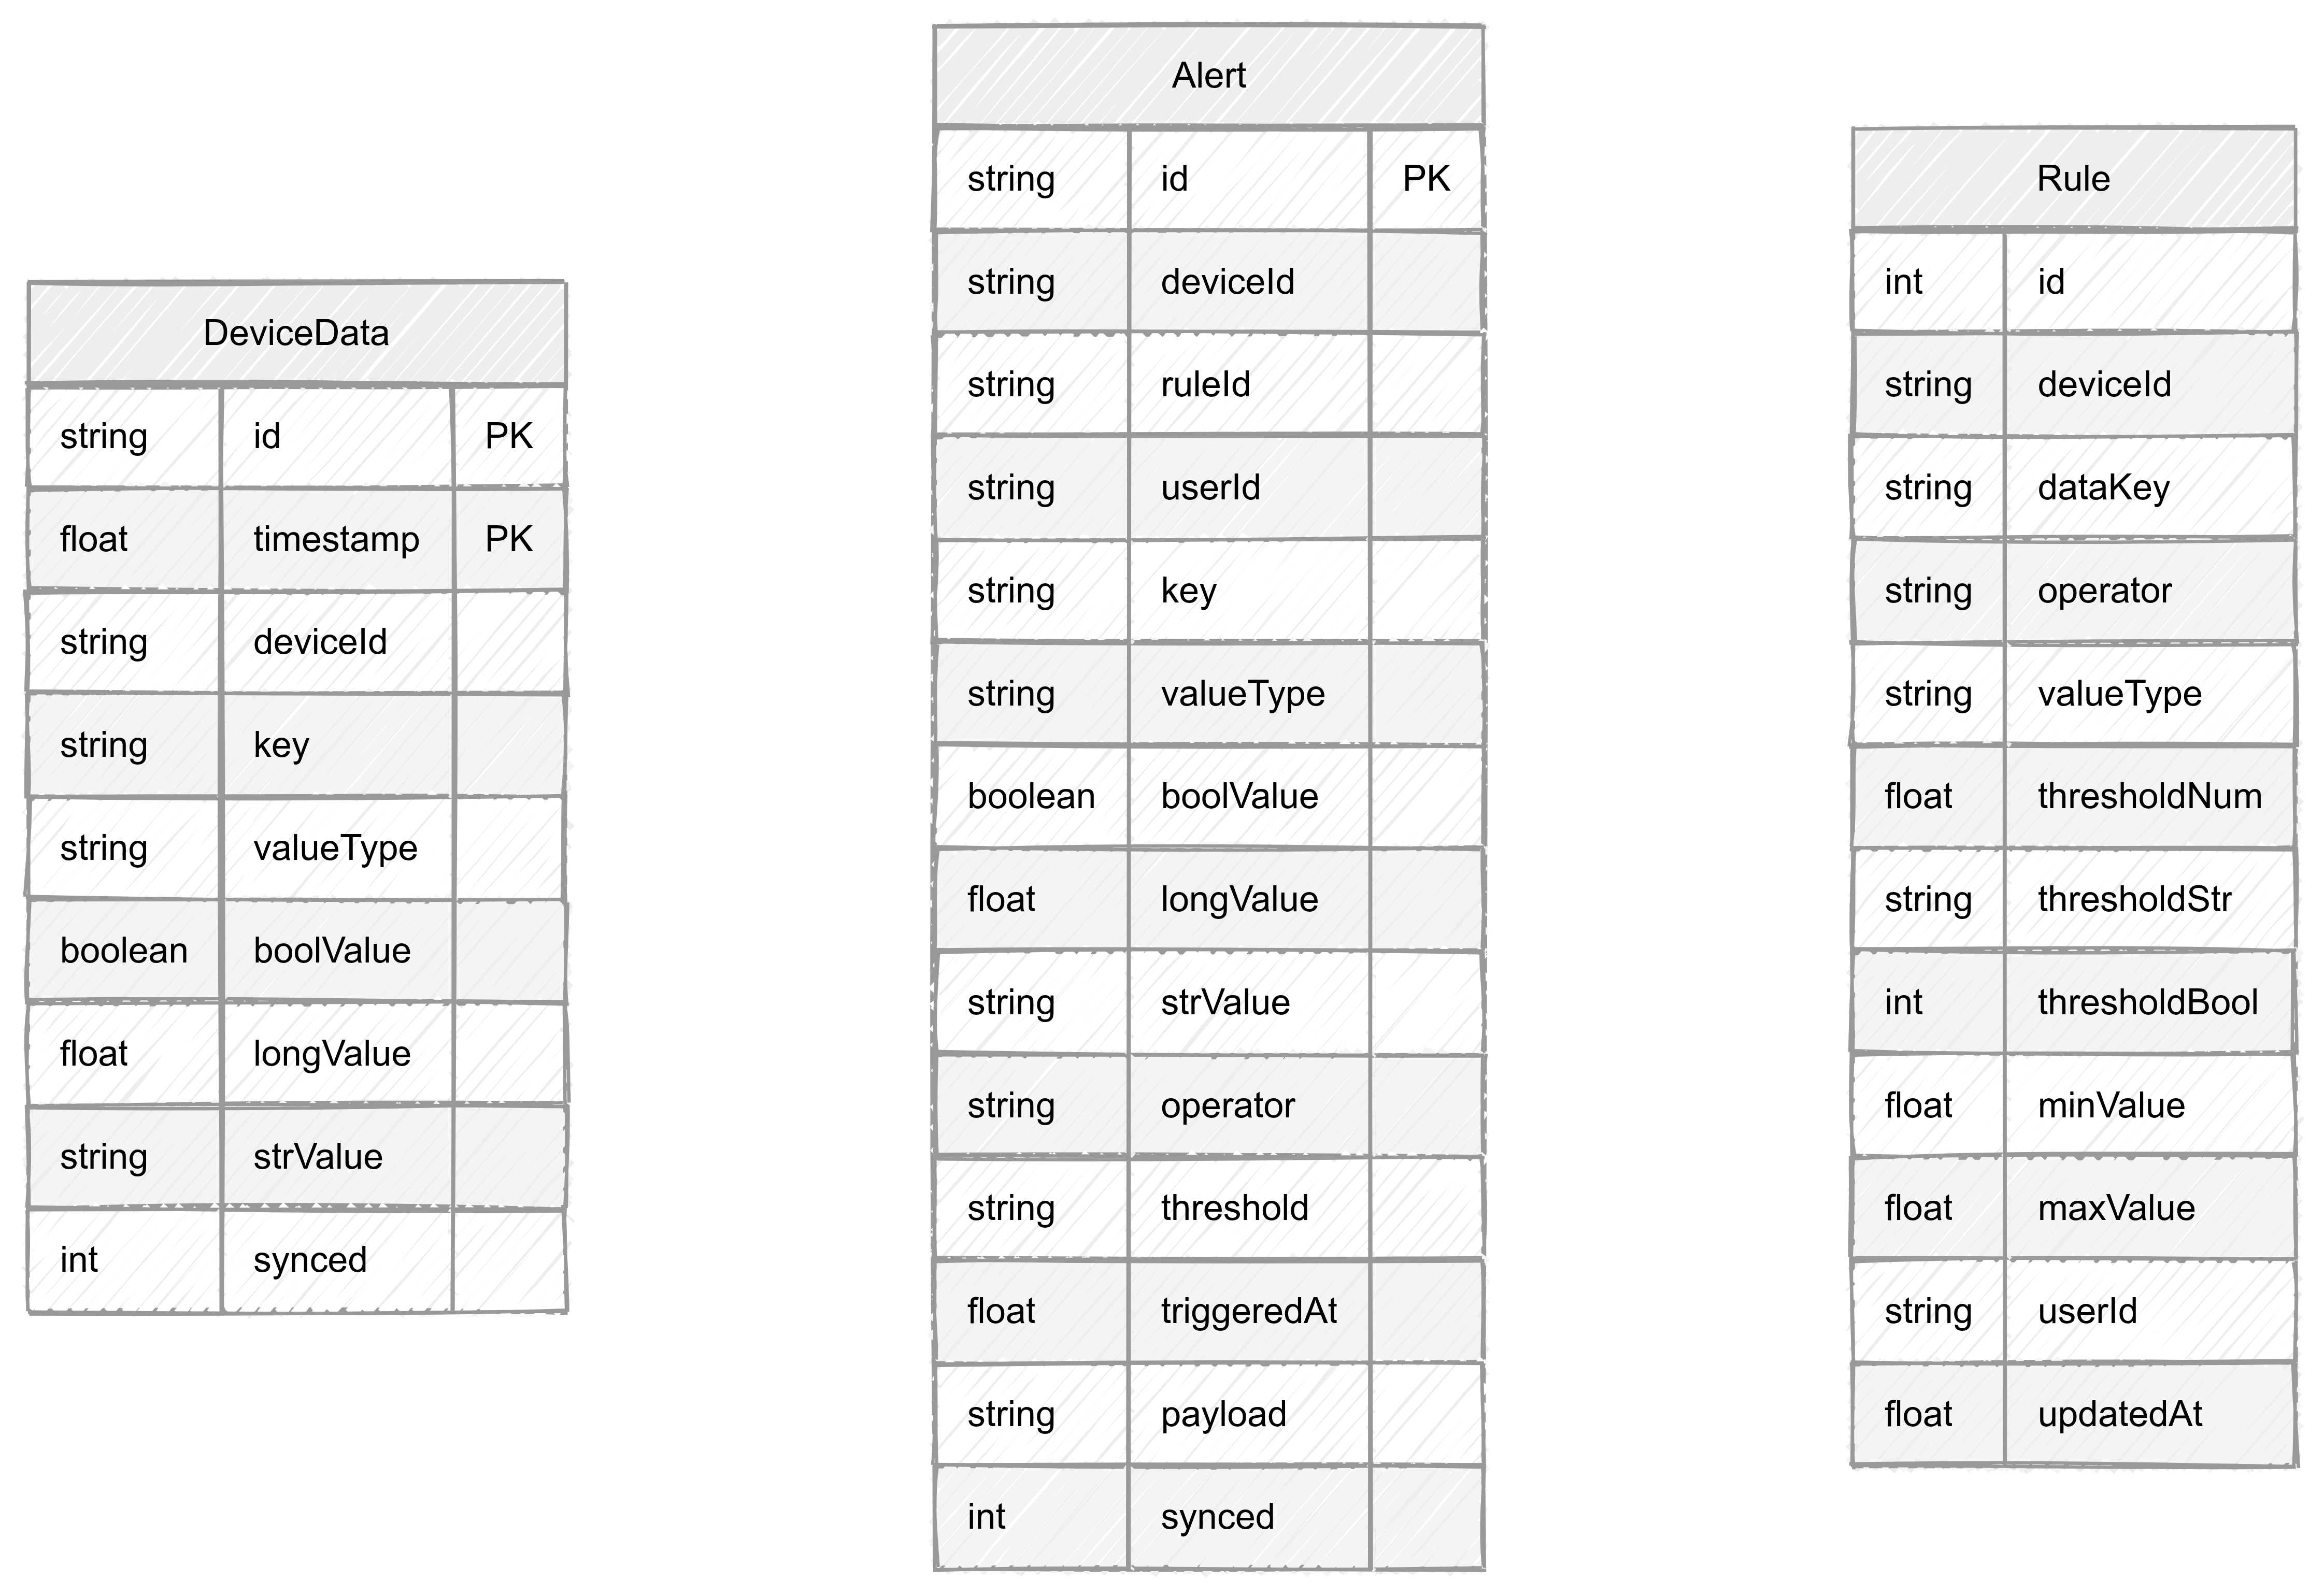
\includegraphics[width=\textwidth, keepaspectratio]{Chapters/Figures/Databases/Implemented/edgeDbSchema.png}
    \caption{Edge node SQLite database schema, showing the three tables used for local telemetry buffering, alert storage, and rule caching.}
    \label{fig:edge-sqlite-schema}
\end{figure}

The data stored in this database is short-lived. After telemetry and alerts are synchronized with the cloud, they are removed to keep the local database small. Rules are replaced on each synchronization cycle instead of being updated one by one, which keeps the local cache aligned with the cloud version.

The \texttt{device\_data} table has an index on \texttt{(synced, timestamp)}, and the \texttt{alerts} table has an index on \texttt{(synced, triggered\_at)}. These indexes help the synchronization process find unsent records in chronological order.
